\documentclass[11pt, letterpaper, landscape]{article}
% Required Packages
\usepackage[T1]{fontenc}
\usepackage[scaled=0.92]{helvet}
\renewcommand{\familydefault}{\sfdefault}

\usepackage{fullpage}
\usepackage{graphicx}
\usepackage{indentfirst}
\usepackage{verbatim}
\usepackage{float}
\usepackage{pdfpages}
\usepackage[font=small,labelfont=bf]{caption}
\usepackage{hyperref}
\usepackage{listings}
\usepackage{color}
\usepackage[tight]{subfigure}
\usepackage{xcolor}
\usepackage{tcolorbox}
\usepackage[export]{adjustbox}
\definecolor{light-gray}{gray}{0.95}

\graphicspath{{figures/}}

\setlength{\parindent}{0pt}
\addtolength{\parskip}{0.4cm}

\begin{document}
\clearpage
\thispagestyle{empty}
\pagestyle{empty}
\small

\includegraphics[height=3.0em]{osrf-pos-horz-pms5265}
\hspace{0.51\textwidth}%

\includegraphics[height=3.0em]{gazebo.pdf}

\begin{center}
{\LARGE HAPTIX Simulation Reference}%
\end{center}

% First row
\begin{figure}[!htb]
  \centering
  \begin{minipage}[t]{0.48\textwidth}
    \begin{tcolorbox}[height=6.5cm,colback=gray!8,colframe=gray!15]
      \section*{Quick Start}
      \begin{enumerate}
        \item Plugin Optitrack, and put on the 3D glasses and forearm markers.\\
          \textcolor{blue}{http://gazebosim.org/haptix/tutorials/optitrack}
        \item Click the Gazebo desktop icon.
        \item Align your arm to roughly match the MPL arm's pose in simulation.
        \item Press the space bar to start motion tracking.
        \item Use keyboard for grasping.
      \end{enumerate}
    \end{tcolorbox}
  \end{minipage}%
  \hspace{0.02\textwidth}%
  \begin{minipage}[t]{0.48\textwidth}
    \begin{tcolorbox}[height=6.5cm,colback=gray!8,colframe=gray!15]
      \section*{Stereo Display \textcolor{blue}{\textnormal{\small http://gazebosim.org/haptix/tutorials/stereo}}}
      Stereo rendering is enable by default, and simulation will look blurry. Use the Nvidia 3D glasses to see simulation in 3D.\\

      {\bf Sync:} With glasses on, press the button on the frame's left side.\\
      {\bf Enable/disable:} Use the {\em Stereo} checkbox in the onscreen GUI.\\
    \end{tcolorbox}
  \end{minipage}
\end{figure}

% Second row
\begin{figure}[!htb]
  \centering
  \begin{minipage}[t]{0.48\textwidth}
    \begin{tcolorbox}[height=5cm,colback=gray!8,colframe=gray!15]
      \section*{Tutorials}
      \begin{itemize}
        \item Install: \textcolor{blue}{http://gazebosim.org/haptix/tutorials/install}
        \item Teleoperation: \textcolor{blue}{http://gazebosim.org/haptix/tutorials/teleop}
        \item Optitrack: \textcolor{blue}{http://gazebosim.org/haptix/tutorials/optitrack}
        \item C-API: \textcolor{blue}{http://gazebosim.org/haptix/tutorials/capi}
        \item Matlab-API: \textcolor{blue}{http://gazebosim.org/haptix/tutorials/matlab}
      \end{itemize}
    \end{tcolorbox}
  \end{minipage}%
  \hspace{0.02\textwidth}%
  \begin{minipage}[t]{0.48\textwidth}
    \begin{tcolorbox}[height=5cm,colback=gray!8,colframe=gray!15]
      \section*{Help and Resources}
      \begin{itemize}
        \item Project page: \textcolor{blue}{http://gazebosim.org/haptix}
        \item API: \textcolor{blue}{http://gazebosim.org/haptix/api}
        \item Questions and answers: \textcolor{blue}{http://answers.gazebosim.org}
        \item Issue tracker: \textcolor{blue}{http://bitbucket.org/osrf/handsim/issues}
        \item Email: \textcolor{blue}{haptix-support@osrfoundation.org}
      \end{itemize}

    \end{tcolorbox}
  \end{minipage}
\end{figure}

% Third row
\begin{figure}[!htb]
  \centering

  \begin{minipage}[t]{0.48\textwidth}
    \begin{tcolorbox}[height=6cm,colback=gray!8,colframe=gray!15]
      \section*{Spacenav \textcolor{blue}{\textnormal{\small http://gazebosim.org/haptix/tutorials/spacenav}}}
      {\bf Purpose:} Control viewpoint and arm position.\\
      {\bf Use:} Press left button, located on base, to toggle between viewpoint and arm control.\\
      \newline
      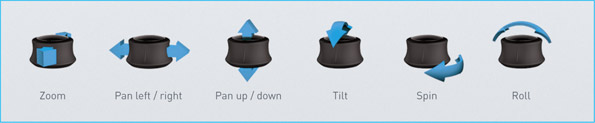
\includegraphics[width=1.0\textwidth]{spacenav_control.jpg}
    \end{tcolorbox}
  \end{minipage}%
  \hspace{0.02\textwidth}%
  \begin{minipage}[t]{0.48\textwidth}
    \begin{tcolorbox}[height=6cm,colback=gray!8,colframe=gray!15]
      \section*{Optitrack \textcolor{blue}{\textnormal{\small http://gazebosim.org/haptix/tutorials/optitrack}}}
      {\bf Purpose:} Control viewpoint and arm position.\\
      {\bf Use:}
      \begin{enumerate}
        \item Make sure Optitrack is plugged in.
        \item Wear the 3D glasses, and arm band. 
        \item Press space bar to enable/disable tracking. 
        \item Make sure the camera can always see the markers.
      \end{enumerate}
    \end{tcolorbox}
  \end{minipage}%

\end{figure}

\begin{minipage}[t]{0.98\textwidth}
  \begin{tcolorbox}[colback=gray!8,colframe=gray!15]

    \section*{Keyboard Teleoperation \textcolor{blue}{\textnormal{\small http://gazebosim.org/haptix/tutorials/teleop}}}

    \begin{figure}[H]
      \centering
      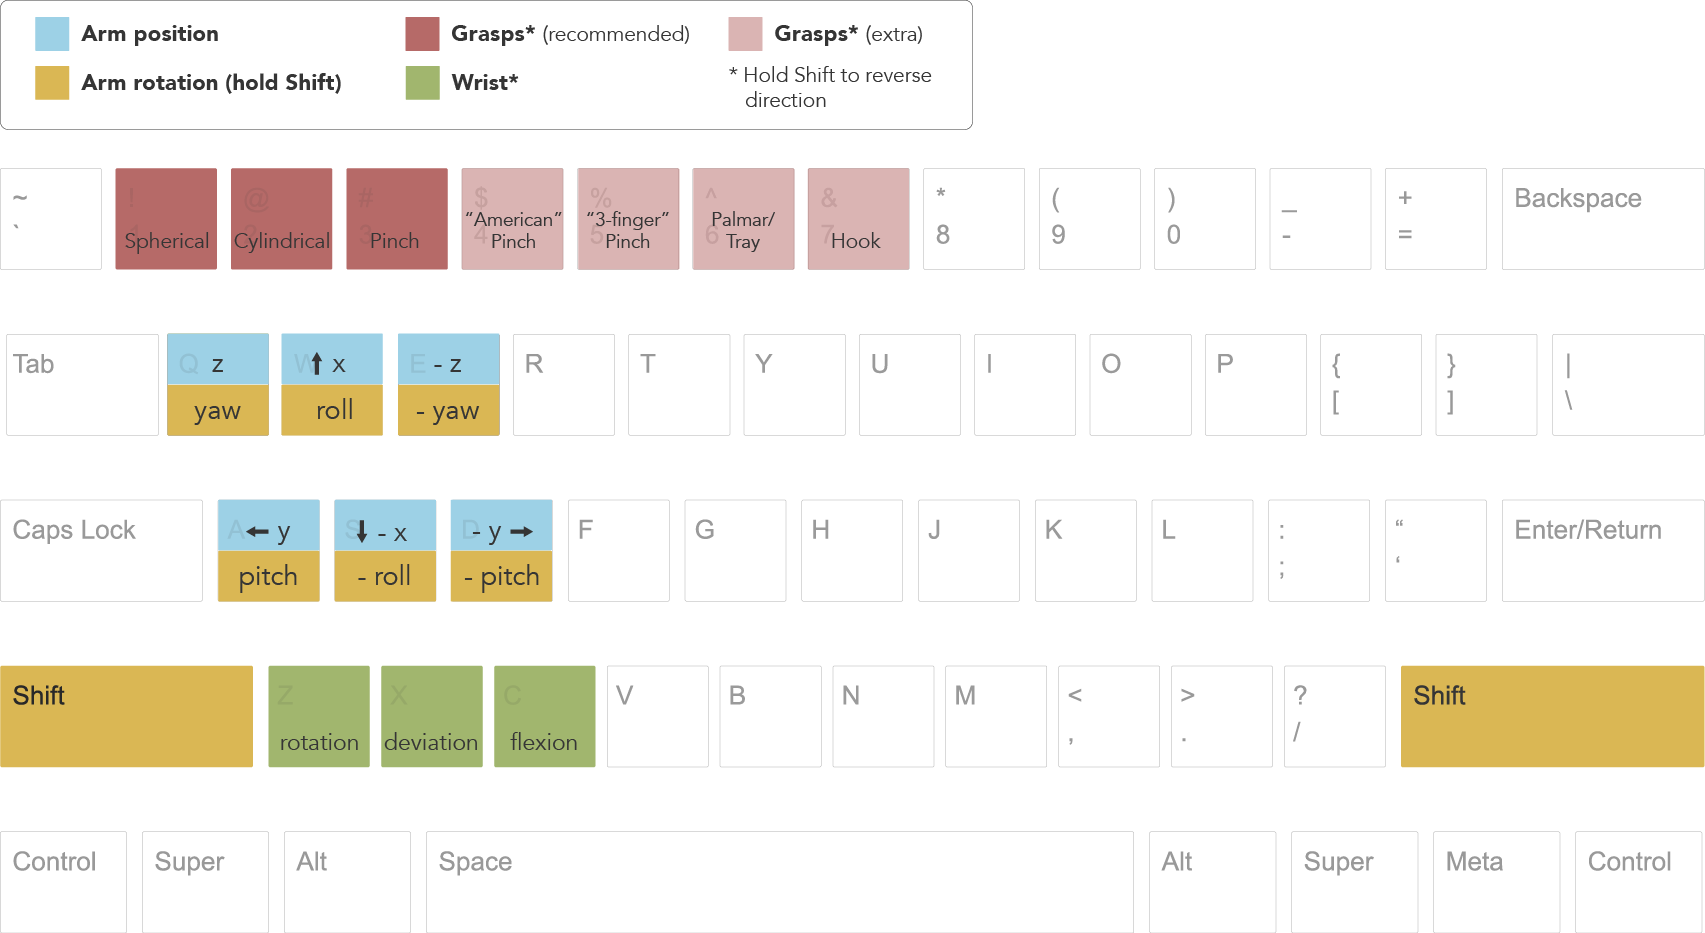
\includegraphics[width=0.8\textwidth]{figures/keyboard.png}
    \end{figure}
  \end{tcolorbox}
\end{minipage}

\end{document}
